\begin{center}
  \section{Calibrazione del monocromatore}
\medskip
\end{center}
{\color{gray}\hrule}
\medskip

Come accennato nella sezione precedente, la scala graduata del monocromatore è in unità arbitrarie (u.a.): la prima parte dell'esperienza è dunque volta alla calibrazione dello strumento, permettendo di associare alle unità arbitrarie il valore effettivo della lunghezza d'onda $\lambda$ da esso selezionata. 

A tale scopo si dispone di uno spettrometro di riferimento USB 2000 accoppiato a una fibra ottica, al cui interno, come per il monocromatore, è presente un reticolo diffrattivo con una buona capacità risolutiva ($600$ linee/mm) per ottenere misure più precise e definite. Il reticolo disperde geometricamente la luce nelle diverse componenti spettrali in ingresso su un array CCD a 2048 pixel (area pari a $14 \text{x}200\mu\text{m}^2$). Risulta quindi necessario prima calibrare lo spettrometro collegandolo tramite la fibra ottica ad una lampada spettrale di Argon e Mercurio\footnote{Modello Ocean Optics HG-2 Mercury Argon Wavelength Calibration Light Source.}, le cui righe di emissione sono note.

Seguono quindi le descrizioni del processo di calibrazione dello spettrometro seguito da quello del monocromatore. 


\subsection{Calibrazione dello spettrometro}
Per poter identificare le righe spettrali della lampada Hg-Ar e ottenere una corrispondenza tra i numeri di canale $\#_{ch}$ e le rispettive lunghezze d’onda $\lambda$, si è acquisito più volte lo spettro di emissione variando l'intervallo di acquisizione per poter osservare anche i picchi minori, avendo però cura di non far saturare quest'ultimi (saturazione a 4095 conteggi). \\ Inoltre, per limitare i disturbi dovuti alla luce ambientale e al rumore elettronico interno, si impostano circa 80 misure ripetute per ciascuno spettro di modo che lo spettro fornito dal software sia in realtà la media delle ottanta acquisizioni.

\subsubsection{Relazione polinomiale per la calibrazione del monocromatore}
Una volta ottenute le diverse acquisizioni dello spettro della lampada Hg-Ar, si sono scelti 10 picchi spettrali, a ciascuno dei quali è stato associato con cura il valore teorico in nanometri della lunghezza d'onda riportato sulla lampada. 

Per ogni picco è stato effettuato un fit gaussiano da cui vengono estratti valore medio $\mu_{\#}$ e deviazione standard $\sigma_{\#}$: tale approccio è sperimentalmente utile ma non è giustificato da alcuna evidenza statistica, per questo motivo come incertezza sui valori medi si utilizza la larghezza a metà altezza $\delta_{\#} = 2\sqrt{2 \ln 2} \cdot \sigma_{\#}$, senza aumentarne significativamente la stima. \\
I valori medi dei picchi $\mu_{\#,i}$ e le rispettive incertezze $\delta_{\#,i}$ sono riportati nella tabella \ref{tab:cal_spettr} in appendice.

Dal grafico delle coppie di valori ($\mu_{\#,i}$,$\lambda_i$) (si veda la figura \ref{fig:cal_spettr}) si ipotizza inizialmente un andamento lineare, tuttavia il modello non viene accettato sui dati; perciò in seconda battuta si è tentato con esito positivo di descrivere i dati con un polinomio di secondo grado. \\

\begin{figure}[H]
    \centering
    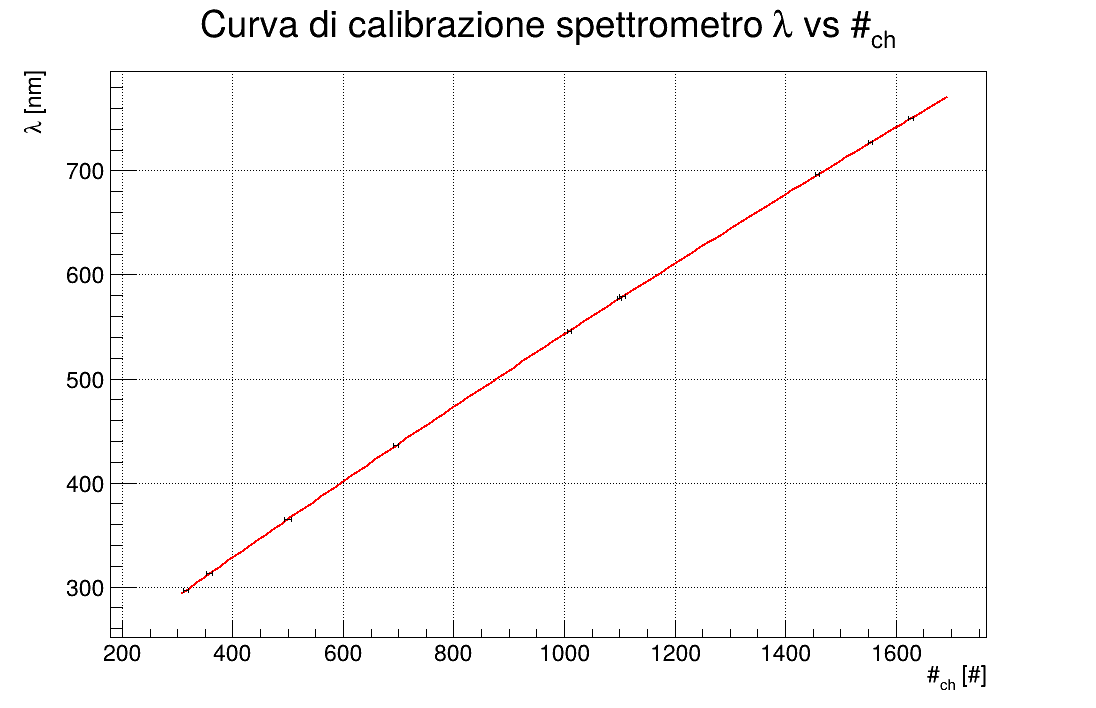
\includegraphics[width=0.85\linewidth]{cal_spettr.png}
    \caption{ \footnotesize Coppie di valori ($\mu_{\#,i}$,$\lambda_i$) e fit polinomiale di secondo grado $y = p_0 + p_1 x + p_2x^2 $ con parametri restituiti: $p_0 =  ( 177 \pm 3) \text{nm}$, $p_1=( 0.388 \pm 0.006) \frac{\text{nm}}{\#}$, $p_2 = ( -2.2 \pm 0.3 ) \frac{\text{nm}}{\#^2}$, $\chi^2 = 0.01$ e d.o.f.=$7$.}
    \label{fig:cal_spettr}
\end{figure}

La curva di calibrazione dello spettrometro risultante è
\begin{equation}
    \lambda (\#_{ch}) = (  177 \pm 3)\text{nm } + ( 0.388 \pm 0.006 )\frac{\text{nm}}{\#} \cdot \#_{ch}  +  (  -2.2 \pm 0.3 ) \frac{\text{nm}}{\#^2} \cdot \#_{ch}^2
    \label{eq:cal_spettr}
\end{equation}
\newpage


\subsection{Calibrazione del monocromatore}
Dopo aver rimosso la lampada Hg-Ar, tramite la fibra ottica si connette lo spettrometro al monocromatore e si visualizza lo spettro acquisito della lampada alogena: in realtà si osserva un solo picco emergente che si sposta lungo la scala di pixel dello spettrometro a mano a mano che si ruota la vite micrometrica.

\subsubsection{Relazione lineare per la calibrazione del monocromatore}
Al fine di ricavare la relazione di calibrazione tra la scala della vite micrometrica e le lunghezze d'onda corrispondenti, sono stati acquisiti 20 spettri muovendo in un unico senso la vite a passi di 10 u.a. all'interno del range [$540$,$730$]u.a. e, analogamente al paragrafo 2.1.1, si ricavano tramite fit gaussiani il valore di pixel atteso $\mu_{\#}$ e la sua incertezza $\delta_{\#} = 2\sqrt{2 \ln 2} \cdot \sigma_{\#}$. \\ I valori attesi dei picchi $\mu_{\#,i}$ e i corrispondenti valori in unità arbitrarie letti sul monocromatore $x_i$ con le rispettive incertezze sono riportati nella tabella \ref{tab:cal_monoc} in appendice. 

Dal grafico delle coppie di valori ($x_i$,$\mu_{\#,i}$) (si veda la figura \ref{fig:cal_monoc}) si evince un andamento lineare, perciò si effettua sui dati un fit lineare. \\

\begin{figure}[H]
    \centering
    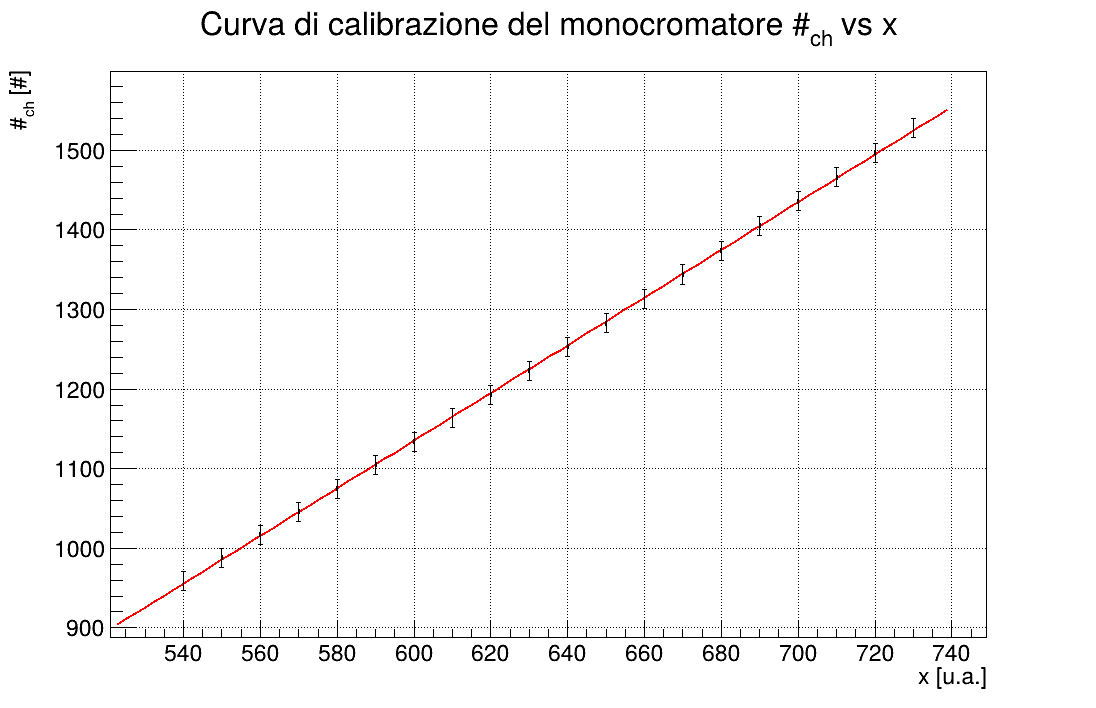
\includegraphics[width=0.85\linewidth]{cal_monoc.png}
    \caption{\footnotesize Coppie di valori ($x_i$,$\mu_{\#}$) e fit lineare $y = p_0 + p_1 x $ con parametri restituiti: $p_0 = (-660 \pm 30)\#$, $p_1= ( 3.00 \pm 0.05) \frac{\#}{\text{u.a.}}$ , $\chi^2 = 0.46$ e d.o.f.=18.}
    \label{fig:cal_monoc}
\end{figure}

La curva di calibrazione del monocromatore risultante è 
\begin{equation}
    \#_{ch} (x) = ( -660 \pm 30)\# + ( 3.00 \pm 0.05 )\frac{\#}{\text{u.a.}} \cdot x
    \label{eq:cal_spettr}
\end{equation}
\newpage